\begin{task}[credit=7]{Regressionsanalyse}
Gegeben sind folgende Datenpunkte:

\begin{table}[h]
\centering
\begin{tabular}{c|cccccccc}
\toprule
\textbf{x} & 1 & 3 & 4 & 6 & 8 & 9 & 11 & 14 \\ \hline
\textbf{y} & 1 & 2 & 4 & 4 & 5 & 7 & 8  & 9  \\
\bottomrule
\end{tabular}
\end{table}

\begin{figure}[h]
\centering
\caption{Veranschaulichung der Datenpunkte zur linearen Regression.}
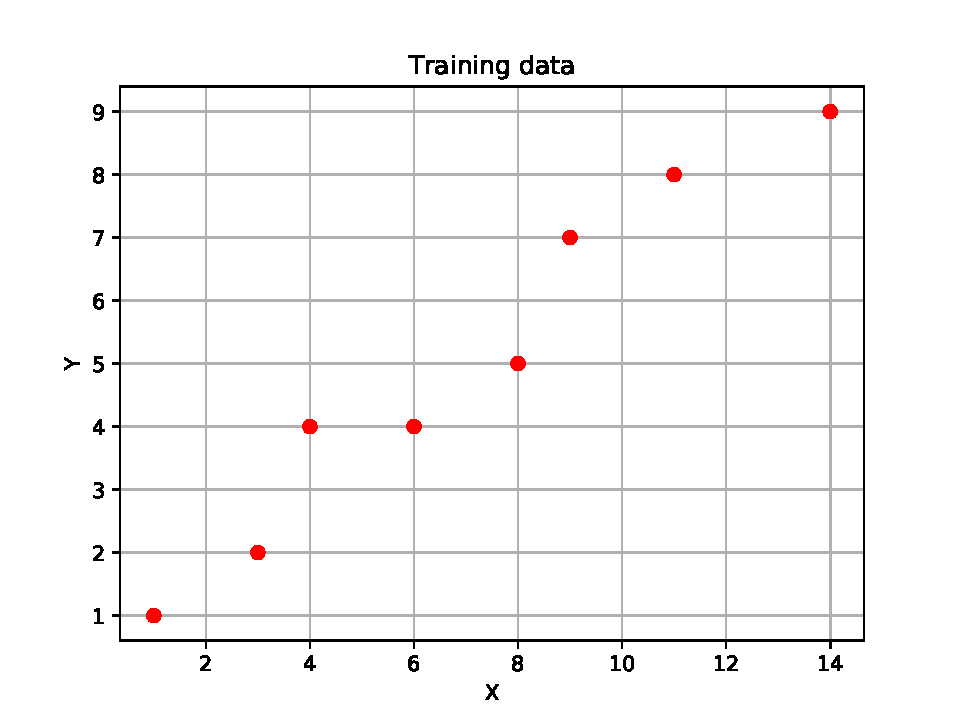
\includegraphics[width=0.5\linewidth]{media/images/data.pdf}
\end{figure}

%We want to build a least square regression model 
Wir möchten eine Regression nach dem Prinzip der kleinsten Fehlrequadrate erstellen:

\begin{equation}
y =f(x)=\left \langle W, x  \right \rangle+b\,.
\end{equation}

Mit der Hilfe eines $(p+1)$-dimensionalen Vektors $\vec{x}=(1, x_1, \cdots , x_p)$ und $x \in \mathbb{R}^{1 \times p}$, können wir $b$ in dem Vektor $W$ codieren:

\begin{equation}
y =f(x)=\left \langle W^{'}, \vec{x}^{T}  \right \rangle,
\end{equation}

wobei hier $W^{'} \in \mathbb{R}^{2 \times 1}$ und $\vec{x} \in \mathbb{R}^{1 \times 2}$.

\begin{subtask}[title=Herleitung,points=5]
 Zeigen Sie, dass das optimale $W^{'}$:
\begin{equation}
W^{'} =  (\vec{X}^{T}\vec{X})^{-1}\vec{X}^{T}Y,
\end{equation}
entspricht, wobei $\vec{X} \in \mathbb{R}^{n \times 2}$ und $Y \in \mathbb{R}^{n \times 1}$.

\begin{solution}
% Geben sie hier ihre Antwort an.
\end{solution}

\end{subtask}


\begin{subtask}[title=Parameterbestimmung,points=2]
Berechnen Sie $W$ und $b$ für den gegebenen Punktdatensatz. Die Inverse $(\vec{X}^{T}\vec{X})^{-1}$ muss dabei nicht manuell berechnet werden.

\begin{solution}
% Geben sie hier ihre Antwort an.
\end{solution}

\end{subtask}
\end{task}
